\documentclass[11]{article}
\usepackage{fullpage, graphicx}

\begin{document}

\section*{Regression Diagnostics in R}
\subsection*{Example: Stack Loss Data}
\begin{verbatim}
> library(MASS)
> data(stackloss)
# Always plot the data!!!
> pairs(stackloss, diag.panel=panel.hist,panel=panel.smooth)
> # see Intro to R for panel.hist function
\end{verbatim}


\centerline{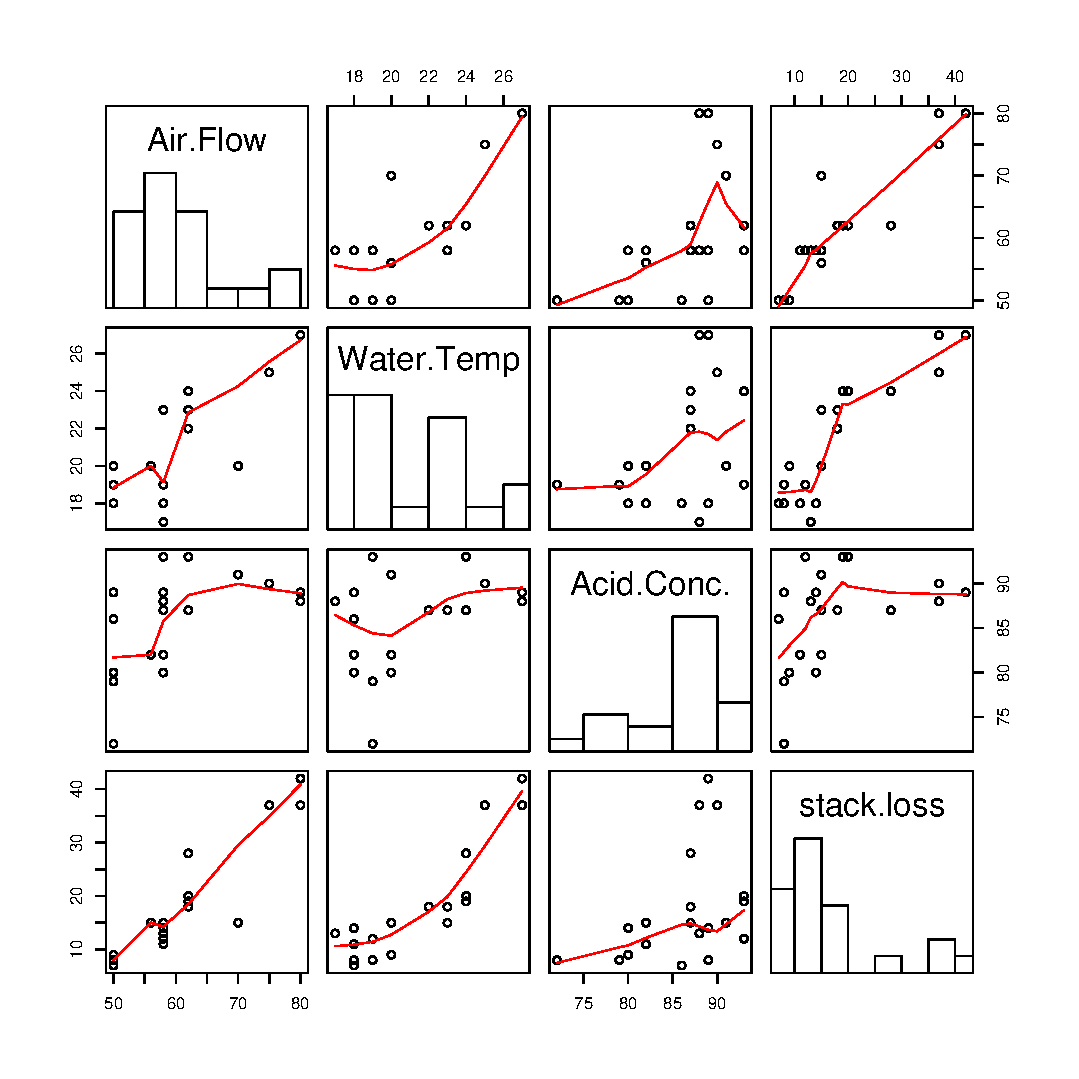
\includegraphics[height=5in]{stackloss-pair.ps}}

\begin{verbatim}
#  Fit the linear model with all variables, no transformations

> stack.lm <- lm(stack.loss ~ ., qr=T, data=stackloss)
> library(car)
> av.plots(stack.lm, ask=F,one.page=T)
> par(mfrow=c(2,2))
> plot(stack.lm)
\end{verbatim}
\newpage
Added variable plots

\centerline{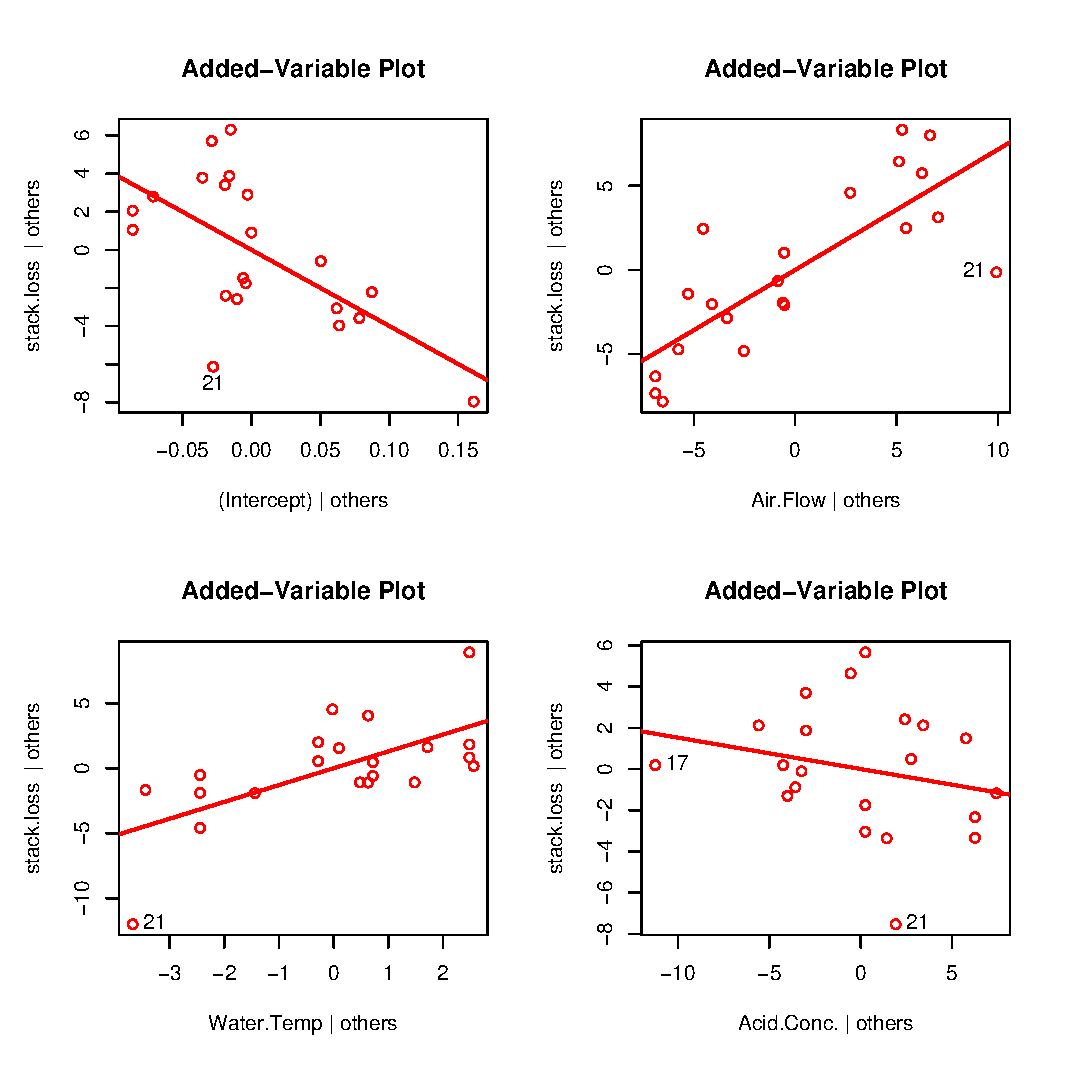
\includegraphics[width=4in]{stackloss-avp.ps}} 

Standard residual plots 

\centerline{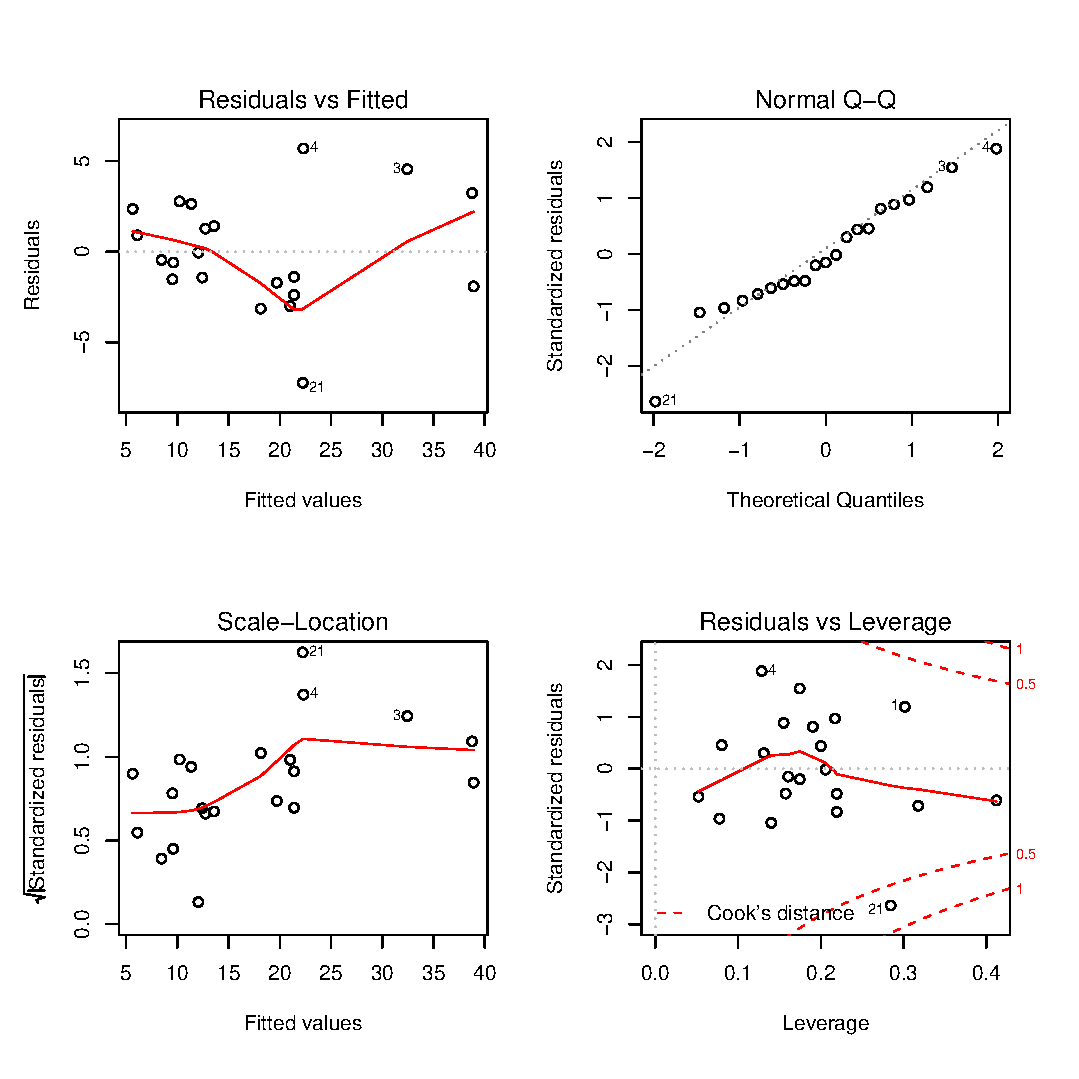
\includegraphics[width=4in]{stackloss-residuals.ps}}

Anything alarming? 


\subsection*{Bayesian Outliers}
Chaloner and Brant declare a point to be an outlier if $P(|\epsilon_i|
> k \sigma)$

Code in Bayes-outliers.R implements the CB diagnostics (please let me know if there are bugs!)  Download the code from the website.  TO load it use the source function.  You will also need the multivariate normal functions from library mvtnorm. Install/load that library if it is not already loaded.

\begin{verbatim}
library(mvtnorm)    
source("bayes-outliers.R")
k = qnorm(.5 + .5*.95^(1/21))
Bout <- Bayes.outlier.prob(stack.lm,k=k)
plot(Bout$prob.outlier, ylab="Posterior Probability of Outlier", xlab="Case", type="h")
abline(h=2*pnorm(-k))
# abline is prior probability of an outlier

indices = outer(1:21, 1:21, FUN=paste)
cbind(indices[Bout$prob.pair.outlier > .0027^2],
      round(Bout$prob.pair.outlier[Bout$prob.pair.outlier > .0027^2],
            digits=6))

      [,1]   [,2]      
 [1,] "3 1"  "0.000129"
 [2,] "4 1"  "3.5e-05" 
 [3,] "21 1" "9e-06"   
 [4,] "1 3"  "0.000129"
 [5,] "4 3"  "9.4e-05" 
 [6,] "21 3" "2.5e-05" 
 [7,] "1 4"  "3.5e-05" 
 [8,] "3 4"  "9.4e-05" 
 [9,] "21 4" "0.002306"
[10,] "1 21" "9e-06"   
[11,] "3 21" "2.5e-05" 
[12,] "4 21" "0.002306"
\end{verbatim}

\centerline{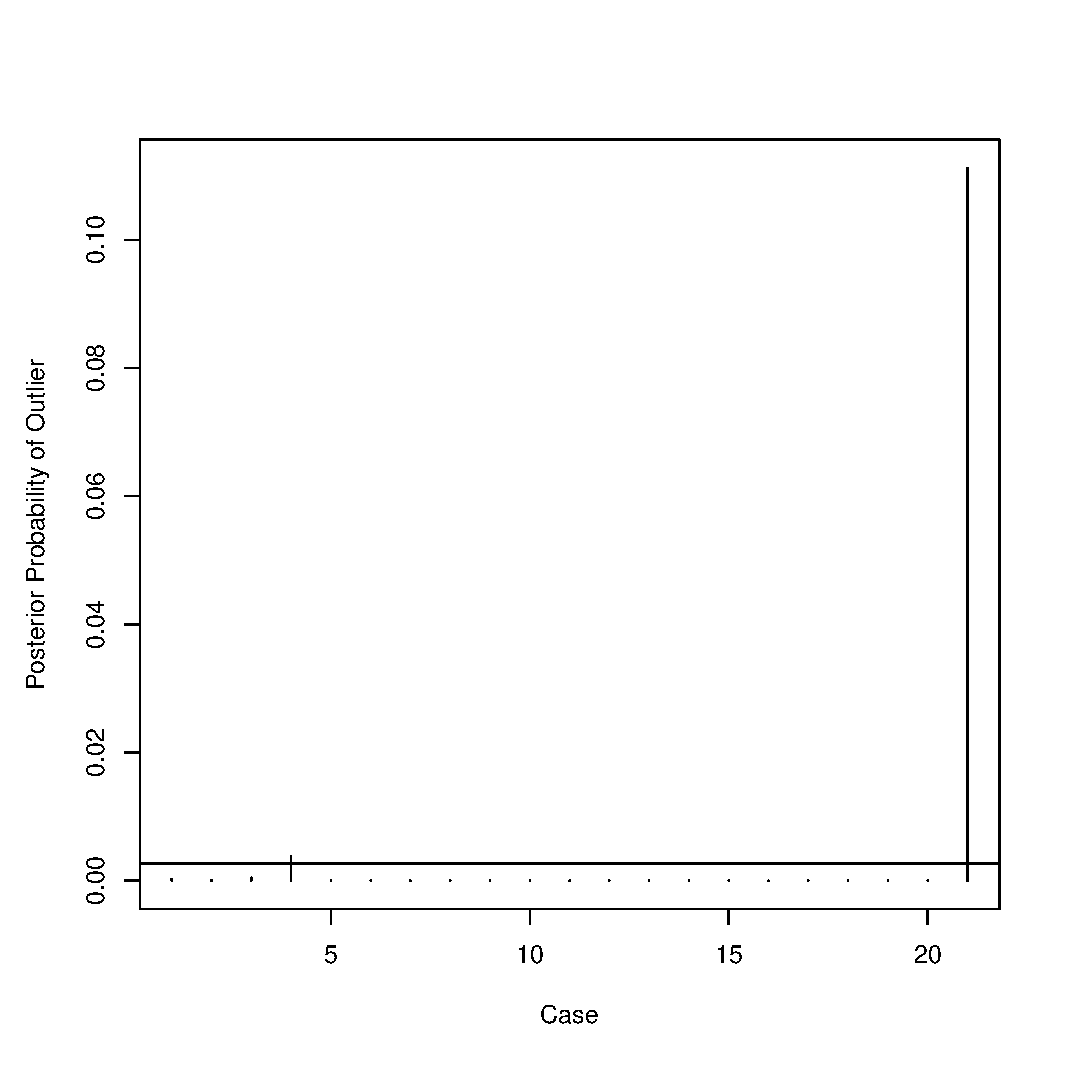
\includegraphics[width=4.5in]{stackloss-bayes.ps}}

\subsection*{Simultaneous Outlier and Variable Selection}
Hoeting, Madigan and Raftery (in various permutations) consider the problem of simultaneous variable selection and outlier identification.  This is implemented in the library(BMA) in the function MC3.REG.
This has the advantage that more than 2 points may be considered as outliers at the same time.
The function uses a Markov chain to identify both important variables and potential outliers, but is coded in Fortran so should run reasonably quickly.

\newpage
\begin{verbatim}
> stack.MC3= MC3.REG(stack.loss, as.matrix(stackloss[, -4]),num.its=10000,
  outliers=TRUE, M0.out=rep(FALSE, 21), outs.list=1:21, M0.var=rep(TRUE, 3))
> summary(stack.MC3)

Call:
MC3.REG(all.y = stack.loss, all.x = as.matrix(stackloss[, -4]),  
   num.its = 10000, M0.var = rep(TRUE, 3), M0.out = rep(FALSE, 21),
   outs.list = 1:21, outliers = TRUE)

Model parameters: PI = 0.1 K = 7 nu = 0.2 lambda = 0.1684 phi = 9.2

  2129  models were selected
 Best  5  models (cumulative posterior probability =  0.4469 ): 

              prob     model 1  model 2  model 3  model 4  model 5
variables                                                         
  Air.Flow    0.99999   x        x        x        x        x     
  Water.Temp  0.61310   x        .        x        x        x     
  Acid.Conc.  0.05236   .        .        .        .        .     
outliers                                                          
  1           0.49631   x        .        .        x        .     
  2           0.06242   .        .        .        .        .     
  3           0.51786   x        .        .        x        .     
  4           0.90962   x        x        x        x        .     
  5           0.01751   .        .        .        .        .     
  6           0.02527   .        .        .        .        .     
  7           0.01902   .        .        .        .        .     
  8           0.01564   .        .        .        .        .     
  9           0.02173   .        .        .        .        .     
  10          0.01664   .        .        .        .        .     
  11          0.01591   .        .        .        .        .     
  12          0.02037   .        .        .        .        .     
  13          0.14446   .        .        .        x        .     
  14          0.05916   .        .        .        .        .     
  15          0.01995   .        .        .        .        .     
  16          0.01379   .        .        .        .        .     
  17          0.01638   .        .        .        .        .     
  18          0.01589   .        .        .        .        .     
  19          0.02402   .        .        .        .        .     
  20          0.04702   .        .        .        .        .     
  21          0.98543   x        x        x        x        x     
                                                                  
post prob              0.18466  0.13627  0.06918  0.03090  0.02589

\end{verbatim}


\end{document}


